\begin{figure}[t]
\centering
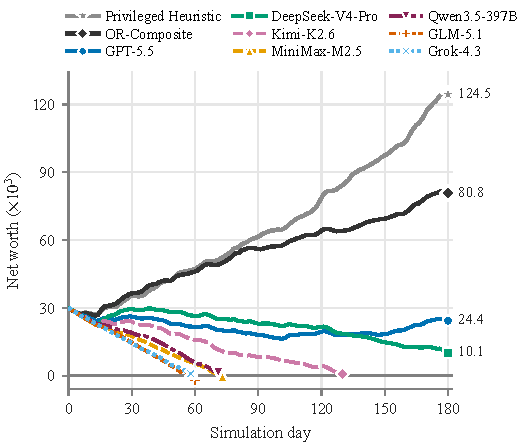
\includegraphics[width=\columnwidth]{figures/net_worth_over_time.pdf}
\caption{Daily net worth trajectories of the two reference
policies and the longest-surviving rollout for each LLM.
Each trajectory terminates when its rollout ends.
Most LLM agents fail to sustain operations over the full
horizon, and even the best-performing agent substantially
underperforms both reference policies in final net worth.
OR-Composite is an operations-research baseline using
only agent-visible information, whereas Oracle is a
privileged reference with access to hidden simulator state.}
\label{fig:net_worth}
\vspace{-2mm}
\end{figure}
% Table 1: comparison with related agent benchmarks (input from introduction.tex so it floats to page 2).
\begin{table*}[t]
\centering
\scriptsize
\setlength{\tabcolsep}{2pt}
\begin{tabular*}{\textwidth}{@{\extracolsep{\fill}}l cc cccc cccc@{}}
\toprule
& \multicolumn{2}{c}{Setting} & \multicolumn{4}{c}{Agent decisions} & \multicolumn{4}{c}{Environment dynamics} \\
\cmidrule(lr){2-3}\cmidrule(lr){4-7}\cmidrule(l){8-11}
Benchmark & Real data & Long-horizon & Pricing & Restock & Supplier & Shelf & Expiry & Reviews & Events & Cash \\
\midrule
WebShop~\citep{3webshopscalablerealworldweb} & \cmark & \xmark & \xmark & \xmark & \xmark & \xmark & \xmark & \pmark & \xmark & \xmark \\
ShoppingBench~\citep{wang2025shoppingbench} & \cmark & \xmark & \xmark & \xmark & \xmark & \xmark & \xmark & \xmark & \xmark & \xmark \\
TheAgentCompany~\citep{xu2024theagentcompany} & \cmark & \pmark & \xmark & \xmark & \xmark & \xmark & \xmark & \xmark & \xmark & \xmark \\
UltraHorizon~\citep{utltabench} & \xmark & \cmark & \xmark & \xmark & \xmark & \xmark & \xmark & \xmark & \xmark & \xmark \\
AIM-Bench~\citep{aimbenchevaluatingdecisionmakingbiases} & \xmark & \pmark & \xmark & \cmark & \pmark & \xmark & \pmark & \xmark & \xmark & \xmark \\
YC-Bench~\citep{he2026ycbench} & \xmark & \cmark & \xmark & \xmark & \xmark & \xmark & \xmark & \xmark & \xmark & \cmark \\
Vending-Bench~\citep{backlund2025vendingbenchbenchmarklongtermcoherence} & \pmark & \cmark & \cmark & \cmark & \cmark & \cmark & \xmark & \xmark & \pmark & \cmark \\
Vending-Bench 2~\citep{andonlabs2025vendingbench2} & \xmark & \cmark & \cmark & \cmark & \cmark & \cmark & \xmark & \pmark & \pmark & \cmark \\
\midrule
\textbf{RetailBench (ours)} & \cmark & \cmark & \cmark & \cmark & \cmark & \cmark & \cmark & \cmark & \cmark & \cmark \\
\bottomrule
\end{tabular*}
\caption{Comparison with related agent benchmarks. Setting: \textbf{Real data} (built on real-world data) and \textbf{Long-horizon} (earlier decisions shape later states over an extended run). Agent decisions: \textbf{Pricing} (set prices), \textbf{Restock} (place replenishment orders), \textbf{Supplier} (choose among suppliers), and \textbf{Shelf} (allocate shelf or slot space). Environment dynamics: \textbf{Expiry} (products expire), \textbf{Reviews} (customer reviews and returns), \textbf{Events} (external demand shocks), and \textbf{Cash} (a cash balance with recurring costs). \cmark{} modeled; \pmark{} partial; \xmark{} absent.}
\label{tab:benchmark_axes}
\vspace{-3mm}
\end{table*}


Large language models (LLMs) with reasoning and tool-use capabilities have made rapid progress on challenging benchmarks for code editing~\citep{swe-bench, tbench_2025}, mathematical and expert-level problem solving~\citep{omni-olpc, hle}, information retrieval~\citep{mialon2023gaiabenchmarkgeneralai, browsecomp}, and web interaction~\citep{webarenarea, mind2web}. However, these benchmark successes often do not translate into equally reliable performance in real-world settings, where agents must sustain coherent decision-making, adapt to evolving conditions, and recover from accumulated errors over extended horizons.

Recent studies reveal substantial limitations in agent reliability in realistic environments, where even leading agents struggle to sustain effective decision-making amid complex operational constraints, evolving conditions, and delayed consequences \citep{kwa2025measuringaiabilitycomplete, metr2025measuring, nof1, andonlabs2025vendingbench2, backlund2025vendingbenchbenchmarklongtermcoherence}. To better capture the complexity of real-world tasks, benchmarks such as OdysseyBench, OSWorld 2.0, EnterpriseOps-Gym, and YC-Bench increasingly evaluate agents in realistic environments involving interconnected decisions, dynamic feedback, and sustained interactions \citep{odysseybenchevaluatingllmagents, yuan2026osworld2,malay2026enterpriseopsgym,he2026ycbench}. However, integrated, data-grounded retail operations remain
underrepresented in existing long-horizon agent evaluations.

To address the limited coverage of integrated, data-grounded
retail operations in existing agent benchmarks, we introduce \textbf{RetailBench}, a controlled, data-grounded benchmark for long-horizon retail operations that captures the complexities of real-world business decision-making. Agents autonomously manage pricing, replenishment, supplier selection, information acquisition, and memory under delivery delays, inventory aging, stockouts, customer feedback, returns, and financial constraints.We evaluate seven LLMs in this realistic retail environment. Figure~\ref{fig:net_worth} reveals substantial gaps in long-horizon operational performance, with only two LLM completing the 180-day horizon. The strongest LLM achieves a final net worth of 24,351 and total sales of 136,405 units, substantially below OR-Composite (80,801 and 202,557), an operations-research reference restricted to agent-visible information (Appendix~\ref{appendix:or_composite}), and the privileged Oracle (124,491 and 263,310). 

To further investigate these performance gaps, we conduct a four-stage analysis of agent trajectories. Our analysis reveals a pronounced disconnect between information acquisition and downstream decision quality: agents demonstrate strong performance in product monitoring and evidence collection, yet struggle to translate acquired evidence into effective decisions and respond promptly to salient operational anomalies amid noisy, high-volume environmental feedback. 
. Our analysis reveals that agents gather evidence effectively but struggle to make high-quality decisions under complex dependencies and respond promptly to operational anomalies. Despite achieving 99.4\% fully evidenced actions, the best-performing agent attains only a 34.8\% high-quality decision rate and a 27.6\% anomaly response rate.

Our main contributions are as follows:

\begin{itemize}[leftmargin=*]
    \item \textbf{A realistic, data-grounded benchmark for long-horizon retail operations.}
    We introduce \textbf{RetailBench}, a controlled, data-grounded environment that captures the complexity of real-world retail operations, where pricing, inventory management, supplier selection, customer feedback, and financial constraints jointly shape long-term outcomes (Section~\ref{sec:env}).

    \item \textbf{Systematic evaluation of agents in realistic, long-horizon settings.}
    We evaluate 19 model--scaffold configurations over a 180-day horizon, revealing substantial limitations in sustained operational performance and large gaps relative to an operations-research reference and a privileged Oracle (Section~\ref{sec:benchmark_results}).

    \item \textbf{Fine-grained diagnosis of long-horizon agent failures.}
    We analyze agent trajectories across four stages: product monitoring, evidence collection, decision-making, and anomaly response. Our findings reveal two recurring failure patterns in realistic operational settings: \textbf{shallow evidence-to-decision integration} and \textbf{limited responsiveness to salient operational anomalies} (Sections~\ref{sec:four_stage_setup} and~\ref{sec:failure_pattern_analysis}).
\end{itemize}